\documentclass[12pt,a4paper]{article}

\usepackage[utf8]{inputenc}
\usepackage[T2A]{fontenc}
\usepackage[ukrainian]{babel}
\usepackage{geometry}
\usepackage{amsmath}
\usepackage{array}
\usepackage{multirow}
\usepackage[table]{xcolor}
\usepackage{makecell}
\usepackage{graphicx}
\usepackage{fancyvrb}
\usepackage{hyperref}

\geometry{
    left=2cm,
    right=2cm,
    top=2cm,
    bottom=2cm
}

\setlength{\parindent}{1.25cm}
\setlength{\parskip}{0.2em}
\setlength{\extrarowheight}{2pt}

\newcolumntype{C}[1]{>{\centering\arraybackslash}p{#1}}
\newcommand{\sectiontitle}[1]{\begin{center} \textbf{\large #1} \end{center}}
\fvset{frame=single, framesep=2mm, fontsize=\small}

\hypersetup{
    unicode=true,
    pdftitle={ІО-41, Давидчук А.М., АК. Частина 1, Лабораторна робота №5},
    pdfauthor={Давидчук Артем},
    pdfsubject={Архітектура Комп'ютерів. Частина 1}
}

\begin{document}

\hypersetup{pageanchor=false}
\begin{titlepage}

        \begin{center}
\includegraphics[width=0.7\textwidth]{../../../TITLES/letterhead.png}\end{center}

        \begin{center}
            \large Національний технічний університет України\\
            «Київський політехнічний інститут імені Ігоря Сікорського»\\[1em]
            Факультет інформатики та обчислювальної техніки\\
            Кафедра обчислювальної техніки
        \end{center}

        \vfill

        \begin{center}
            \textbf{\LARGE Архітектура Комп'ютерів. Частина 1}\\[2em]
            \textbf{\Large Лабораторна робота №5}\\[0.5em]
            «Формування системи команд процесора, розробка програм і мікропрограм обробки інформації в ЕОМ»
        \end{center}

        \vfill

        \begin{flushright}
            Виконав: студент 2 курсу ФІОТ, гр. ІО-41\\
            \textit{Давидчук А. М.}\\
            Залікова книжка № 4106\\[1em]
            Перевірив: \textit{Верба О.\,А.}
        \end{flushright}

        \vfill

        \begin{center}Київ --- 2026\end{center}

    \end{titlepage}
\hypersetup{pageanchor=true}

    \noindent
    \textbf{\underline{Тема:}} «Формування системи команд процесора, розробка програм і мікропрограм обробки інформації в ЕОМ».

    \vspace{1em}

\noindent
\textbf{\underline{Мета:}} навчитися створювати системи команд процесорів, розробляти
алгоритми, програми і мікропрограми обчислення функцій, використовувати
двоадресні команди з регістровою адресацією та вводити дані з пристрою
вводу-виводу.

\begin{center} \textbf{\large Хід роботи} \end{center}

\sectiontitle{Підготовка до роботи}

Номер варіанту -- $4106_{10} = 0001\ 0000\ 0000\ 1010_2$.

\[
a_7 = 0,\quad a_6 = 0,\quad a_5 = 0,\quad a_4 = 1,\quad
a_3 = 0,\quad a_2 = 1,\quad a_1 = 0.
\]

Для визначення варіанта лабораторної роботи використовуються біти
$a_7, a_6, a_5, a_3, a_1$. За комбінацією $a_5a_3a_1 = 000$ необхідно
виконати операції з кодами 0, 1, 2 з таблиці методичних вказівок.

\begin{center}
\small
\begin{minipage}[t]{0.47\textwidth}
\centering
\resizebox{\linewidth}{!}{
\begin{tabular}{|C{1.1cm}|C{1.1cm}|C{1.1cm}|C{3.8cm}|}
    \hline
    $a_5$ & $a_3$ & $a_1$ & Операції \\ \hline
    \rowcolor{yellow!25}
    0 & 0 & 0 & 0, 1, 2 \\ \hline
    0 & 0 & 1 & 0, 2, 4 \\ \hline
    0 & 1 & 0 & 3, 4, 2 \\ \hline
    0 & 1 & 1 & 2, 3, 5 \\ \hline
\end{tabular}
}
\end{minipage}
\hfill
\begin{minipage}[t]{0.47\textwidth}
\centering
\resizebox{\linewidth}{!}{
\begin{tabular}{|C{1.1cm}|C{1.1cm}|C{1.1cm}|C{1.5cm}|C{1.5cm}|}
    \hline
    $a_7$ & $a_6$ & $a_5$ & РС & РД \\ \hline
    \rowcolor{yellow!25}
    0 & 0 & 0 & 02H & 04H \\ \hline
    0 & 0 & 1 & 12H & 14H \\ \hline
    0 & 1 & 0 & 22H & 24H \\ \hline
    0 & 1 & 1 & 32H & 34H \\ \hline
\end{tabular}
}
\end{minipage}

\vspace{1.2em}

\begin{minipage}[t]{0.6\textwidth}
\centering
\resizebox{\linewidth}{!}{
\begin{tabular}{|C{1.5cm}|C{3.2cm}|C{3.2cm}|}
    \hline
    Код & Операція & Функція \\ \hline
    \rowcolor{yellow!25}
    0 & $X + Y$ & $F_1 = X + Y$ \\ \hline
    \rowcolor{yellow!25}
    1 & $X - Y$ & $F_2 = X - Y$ \\ \hline
    \rowcolor{yellow!25}
    2 & $X \wedge Y$ & $F_3 = X \wedge Y$ \\ \hline
    3 & $X \vee Y$ & -- \\ \hline
    4 & $X \oplus Y$ & -- \\ \hline
\end{tabular}
}
\end{minipage}
\end{center}
\normalsize

Операнд $X$ вводиться з пристрою введення через регістр даних ЗП, операнд
$Y$ розміщується в оперативній пам'яті. Результати $F_1$, $F_2$ та $F_3$
записуються в ОП. Операнди подаються у доповняльному коді, розрядність
операндів -- 16 біт з двома знаковими розрядами.

\newpage

\sectiontitle{Структура ЕОМ}

\begin{center}
    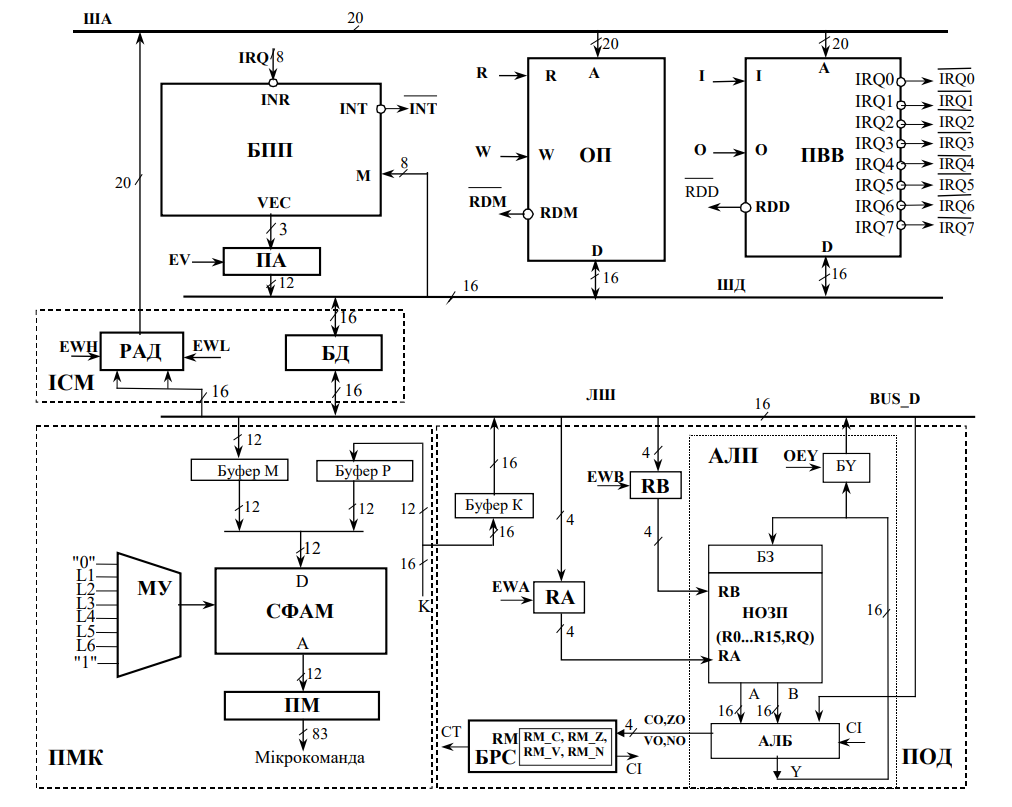
\includegraphics[width=0.82\textwidth]{../lab3/media/eom.png}
\end{center}

\sectiontitle{Формат команд та регістрів стану і даних}

\begin{center}
\small
\begin{tabular}{|C{2.2cm}|C{2.5cm}|C{2cm}|C{7cm}|}
    \hline
    \textbf{Поле} & \textbf{Біти} & \textbf{Довжина} & \textbf{Призначення} \\ \hline
    $F$ & 15 & 1 & формат команди: 0 -- одноадресна, 1 -- двоадресна \\ \hline
    $OP$ & 14--11 & 4 & код операції \\ \hline
    $TA$ & 10 & 1 & тип адресації: 0 -- пряма, 1 -- пряма регістрова \\ \hline
    $A$ & 9--0 & 10 & адреса ОП, адреса порту або поля адрес регістрів \\ \hline
\end{tabular}
\end{center}

\begin{center}
\small
\begin{tabular}{|C{1.6cm}|C{10cm}|}
    \hline
    \textbf{Регістр} & \textbf{Призначення} \\ \hline
    РС & 7-й біт містить ознаку готовності пристрою до обміну даними \\ \hline
    РД & містить дані, що зчитуються із зовнішнього пристрою \\ \hline
\end{tabular}
\end{center}
\normalsize

\newpage

\sectiontitle{Архітектура системи}

\begin{center}
\begin{minipage}[t]{0.47\textwidth}
\centering
\textbf{Структура НОЗП}

\vspace{0.4em}
\small
\begin{tabular}{|C{1.8cm}|p{4.5cm}|}
    \hline
    \textbf{Регістр} & \textbf{Призначення} \\ \hline
    R1 & операнд $X$ \\ \hline
    R2 & операнд $Y$ \\ \hline
    R3 & регістр команди \\ \hline
    R4 & лічильник команд \\ \hline
    R5 & стан зовнішнього пристрою \\ \hline
    R6 & результат $F_1 = X + Y$ \\ \hline
    R7 & результат $F_2 = X - Y$ \\ \hline
    R8 & результат $F_3 = X \wedge Y$ \\ \hline
\end{tabular}
\end{minipage}
\hfill
\begin{minipage}[t]{0.47\textwidth}
\centering
\textbf{Структура ПМК}

\vspace{0.4em}
\small
\begin{tabular}{|C{1.5cm}|p{4.7cm}|}
    \hline
    \textbf{Адреса} & \textbf{Мікропрограма} \\ \hline
    0h & START \\ \hline
    1h & TEST\_ZP \\ \hline
    2h & Z\_JUMP \\ \hline
    3h & INPUT\_X \\ \hline
    4h & GET\_Y \\ \hline
    5h & X\_ADD\_Y \\ \hline
    6h & WRITE\_F1 \\ \hline
    7h & X\_SUB\_Y \\ \hline
    8h & WRITE\_F2 \\ \hline
    9h & X\_AND\_Y \\ \hline
    Ah & WRITE\_F3 \\ \hline
    Bh & END \\ \hline
\end{tabular}
\end{minipage}
\end{center}

\vspace{1em}

\begin{center}
\begin{minipage}[t]{0.47\textwidth}
\centering
\textbf{Структура ОП}

\vspace{0.4em}
\small
\begin{tabular}{|C{1.5cm}|p{4.8cm}|}
    \hline
    \textbf{Адреса} & \textbf{Вміст} \\ \hline
    0h & резерв \\ \hline
    1h & значення $Y$ \\ \hline
    2h & результат $F_1$ \\ \hline
    3h & результат $F_2$ \\ \hline
    4h & результат $F_3$ \\ \hline
    10h--1Ah & програма \\ \hline
\end{tabular}
\end{minipage}
\hfill
\begin{minipage}[t]{0.47\textwidth}
\centering
\textbf{Структура ЗП}

\vspace{0.4em}
\small
\begin{tabular}{|C{1.5cm}|p{4.8cm}|}
    \hline
    \textbf{Адреса} & \textbf{Вміст} \\ \hline
    02h & РС, регістр стану \\ \hline
    04h & РД, регістр даних \\ \hline
\end{tabular}
\end{minipage}
\end{center}

\newpage

\sectiontitle{Змістовний алгоритм}

\begin{center}
    
\includegraphics[width=0.72\textwidth]{media/alg.png}
\end{center}

\newpage

\sectiontitle{Система команд}

\begin{center}
\small
\begin{tabular}{|C{2.5cm}|C{2cm}|p{8cm}|}
    \hline
    \textbf{Команда} & \textbf{Код операції} & \textbf{Операція} \\ \hline
    \texttt{TEST\_ZP} & 1h & зчитування РС зовнішнього пристрою та перевірка готовності \\ \hline
    \texttt{Z\_JUMP} & 2h & умовний перехід до адреси з поля команди \\ \hline
    \texttt{INPUT\_X} & 3h & введення операнда $X$ з РД зовнішнього пристрою \\ \hline
    \texttt{GET\_Y} & 4h & зчитування операнда $Y$ з оперативної пам'яті \\ \hline
    \texttt{X\_ADD\_Y} & 5h & двоадресна регістрова команда додавання $X + Y$ \\ \hline
    \texttt{WRITE\_F1} & 6h & запис результату $F_1$ в ОП \\ \hline
    \texttt{X\_SUB\_Y} & 7h & двоадресна регістрова команда віднімання $X - Y$ \\ \hline
    \texttt{WRITE\_F2} & 8h & запис результату $F_2$ в ОП \\ \hline
    \texttt{X\_AND\_Y} & 9h & двоадресна регістрова команда логічного І $X \wedge Y$ \\ \hline
    \texttt{WRITE\_F3} & Ah & запис результату $F_3$ в ОП \\ \hline
    \texttt{END} & Bh & завершення програми \\ \hline
\end{tabular}
\end{center}

\sectiontitle{Програма в оперативній пам'яті}

\begin{center}
\small
\begin{tabular}{|C{1.5cm}|C{4cm}|p{7cm}|}
    \hline
    \textbf{Адреса} & \textbf{Код команди} & \textbf{Мнемоніка} \\ \hline
    10h & \texttt{0802h} & \texttt{TEST\_ZP 02h} \\ \hline
    11h & \texttt{1010h} & \texttt{Z\_JUMP 10h} \\ \hline
    12h & \texttt{1804h} & \texttt{INPUT\_X 04h} \\ \hline
    13h & \texttt{2001h} & \texttt{GET\_Y 01h} \\ \hline
    14h & \texttt{AC62h} & \texttt{X\_ADD\_Y R2, R6} \\ \hline
    15h & \texttt{3002h} & \texttt{WRITE\_F1 02h} \\ \hline
    16h & \texttt{BC72h} & \texttt{X\_SUB\_Y R2, R7} \\ \hline
    17h & \texttt{4003h} & \texttt{WRITE\_F2 03h} \\ \hline
    18h & \texttt{CC82h} & \texttt{X\_AND\_Y R2, R8} \\ \hline
    19h & \texttt{5004h} & \texttt{WRITE\_F3 04h} \\ \hline
    1Ah & \texttt{5800h} & \texttt{END} \\ \hline
\end{tabular}
\end{center}
\normalsize

\newpage

\sectiontitle{Обрахунки}

Для першої перевірки обрано:
\[
X = -2_{10} = FFFE_{16},\qquad Y = 52_{10} = 0034_{16}.
\]
\[
F_1 = X + Y = -2 + 52 = 50_{10} = 0032_{16},
\]
\[
F_2 = X - Y = -2 - 52 = -54_{10} = FFCA_{16},
\]
\[
F_3 = X \wedge Y = FFFE_{16} \wedge 0034_{16} = 0034_{16}.
\]

Для другої перевірки обрано:
\[
X = -10_{10} = FFF6_{16},\qquad Y = -4_{10} = FFFC_{16}.
\]
\[
F_1 = X + Y = -10 - 4 = -14_{10} = FFF2_{16},
\]
\[
F_2 = X - Y = -10 - (-4) = -6_{10} = FFFA_{16},
\]
\[
F_3 = X \wedge Y = FFF6_{16} \wedge FFFC_{16} = FFF4_{16}.
\]

\sectiontitle{Мікропрограма}

\VerbatimInput{src/code.ASM}

\sectiontitle{Результат виконання}

\noindent
Після виконання мікропрограми в оперативній пам'яті мають бути записані:

\begin{center}
\begin{tabular}{|C{3cm}|C{4cm}|C{4cm}|}
    \hline
    \textbf{Адреса} & \textbf{Перша перевірка} & \textbf{Друга перевірка} \\ \hline
    \texttt{M[2h]} & \texttt{0032h} & \texttt{FFF2h} \\ \hline
    \texttt{M[3h]} & \texttt{FFCAh} & \texttt{FFFAh} \\ \hline
    \texttt{M[4h]} & \texttt{0034h} & \texttt{FFF4h} \\ \hline
\end{tabular}
\end{center}

\noindent
Результат виконання для $X = FFFEh$ та $Y = 0034h$:

\begin{center}

\includegraphics[width=0.82\textwidth]{media/demo1.png}
\end{center}

\noindent
Результат виконання для $X = FFF6h$ та $Y = FFFCh$:

\begin{center}

\includegraphics[width=0.82\textwidth]{media/demo2.png}
\end{center}

\noindent
Як видно зі скріншотів, отримані значення в оперативній пам'яті збігаються з
ручними обрахунками.

\sectiontitle{Висновок}

У результаті виконання лабораторної роботи було сформовано систему команд
процесора для обчислення трьох функцій $F_i = (X \circ Y)$, розроблено програму
в машинних кодах і мікропрограму на мнемонічному мікроасемблері. Для мого
варіанта реалізовано операції $X + Y$, $X - Y$ та $X \wedge Y$. Операнд $X$
зчитується із зовнішнього пристрою після програмної перевірки біта готовності,
операнд $Y$ зчитується з оперативної пам'яті, а результати записуються назад в
ОП. Працездатність програми перевірено для двох наборів вхідних даних; отримані
результати збігаються з ручними розрахунками.

\sectiontitle{Відповіді на контрольні питання}

\begin{enumerate}
    \item \textbf{Охарактеризуйте етап дешифрування (розпакування) команд.}

    На етапі дешифрування команда зчитується з оперативної пам'яті до регістра
    команд, після чого з її полів виділяються формат, код операції, тип адресації
    та адресне поле. Код операції використовується для переходу до відповідної
    мікропрограми в ПМК, а адресне поле -- для формування адреси операнда або
    вибору регістрів при прямій регістровій адресації.

    \item \textbf{Як сформувати двоадресну команду при прямій регістровій адресації?}

    При прямій регістровій адресації адресне поле не використовується повністю
    для адреси ОП, тому його можна поділити на два підполя адрес регістрів.
    Наприклад, молодші біти поля команди подаються на RA, а старші -- на RB.
    Так формується команда, яка задає одразу два регістрові операнди.

    \item \textbf{Як забезпечити зчитування і запис даних у пам'ять з урахуванням швидкодії пам'яті?}

    Після встановлення адреси на шині та формування сигналу читання або запису
    процесор повинен чекати сигналу готовності пам'яті \texttt{RDM}. Якщо пам'ять
    ще не готова, мікропрограма залишається в циклі очікування. Це узгоджує
    швидкодію процесора і пам'яті та запобігає зчитуванню або запису некоректних
    даних.

    \item \textbf{Як записати інформацію в RA і RB, навіщо використовуються зазначені регістри?}

    Інформація в RA і RB записується під час розпакування команди за допомогою
    керуючих сигналів \texttt{load RA} і \texttt{load RB} або через макрокоманду,
    що виконує розкодування адресних полів. RA і RB зберігають адреси регістрів
    НОЗП, які підключаються до входів АЛП, тому вони потрібні для виконання
    регістрових двоадресних команд.

    \item \textbf{Поясніть призначення директиви мікроасемблера MACRO.}

    Директива \texttt{MACRO} дозволяє описати власну мнемонічну мікрокоманду,
    яка розгортається в одну або кілька мікрооперацій. Її використовують для
    повторюваних дій, наприклад інкременту лічильника команд або формування
    адреси, щоб зробити мікропрограму коротшою і зрозумілішою.

    \item \textbf{Як забезпечити обмін даними між процесором і ЗП в програмному режимі?}

    У програмному режимі процесор спочатку звертається до регістра стану ЗП і
    перевіряє біт готовності. Якщо пристрій готовий, виконується читання з
    регістра даних або запис у нього за допомогою сигналів \texttt{I}/\texttt{O}
    і очікування сигналу \texttt{RDD}. Якщо пристрій не готовий, програма виконує
    умовний перехід до повторної перевірки.
\end{enumerate}

\end{document}
